\documentclass[openany, 12pt]{report}
\usepackage{documentation}
\usepackage{geometry}
\geometry{
a4paper, 
total={170mm, 257mm},
left=25mm,
top=30mm,
right=25mm,
bottom=20mm,
}
\graphicspath{ {./img/} }

\newcommand{\CourseTitle}{Configuratore auto}
\newcommand{\SubTitle}{Esame di Ingegneria del Software}
\newcommand{\Date}{A.A. 2023-2024 - Settembre 2024}
\newcommand{\Authors}{BIANCHEDI Pietro \\ISELLE Niccol\`o}


\begin{document}
\begin{titlepage}
\centering
\textsc{Universit\`a degli Studi di Verona}
\par\vspace{0.5cm}
\rmfamily
Dipartimento di Informatica \\
\par\vspace{3.5cm}
\textbf{\Huge{\underline{\CourseTitle}}}
\par\vspace{1cm}
\textit{\Large{\SubTitle}}
\par\vspace{0.5cm}
\textit{\large{\Date}}
\par\vspace{4cm}
\textsc{\Authors}
\par\vspace{1cm}
\vfill
\end{titlepage}
\tableofcontents

\chapter{Analisi dei requisiti }

\section{Introduzione}

Il sistema informatico commissionato propone una piattaforma di configurazione e acquisto di automobili per conto di un
gruppo multi-concessionaria. L'utilizzo da parte dei potenziali \textbf{clienti} prevede la possibilit\`a di configurare
l'automobile desiderata, partendo dai modelli di serie proposti e consentendo l'aggiunta di optional e altri parametri di
personalizzazione. Inoltre, \`e possibile per un cliente registrato, richiedere un preventivo e confermare la volont\`a di
acquisto dell'automobile attraverso il sistema. In fase di richiesta del preventivo il cliente pu\`o anche richiedere una
valutazione dell'usato, caricando delle fotografie della sua automobile.

I \textbf{venditori} del gruppo accedendo al sistema possono visualizzare le informazioni riguardanti la loro sede fisica.
I preventivi con annessa una richiesta di valutazione dell'usato devono essere evasi da un impiegato, mentre i preventivi
senza richiesta di valutazione sono evasi automaticamente alla conferma di acquisto da parte del cliente, che dovr\`a anche
decidere la sede di ritiro.
I venditori hanno anche il compito di gestire gli ordini e avvisare i clienti quando l'automobile \`e pronta per il ritiro. 

L'ultima categoria di utenti prevista per il sistema \`e la componente amministrativa del gruppo multi-concessionaria.
Gli \textbf{impiegati} della segreteria hanno il compito di inserire le informazioni sui modelli di automobili e sugli
optional per ogni marca. Inoltre, l'accesso al sistema di questo tipo di utente permette di visualizzare tutti i preventivi
attivi per cliente, marca o per negozio di consegna.

\section{Casi d'uso}

\begin{center}
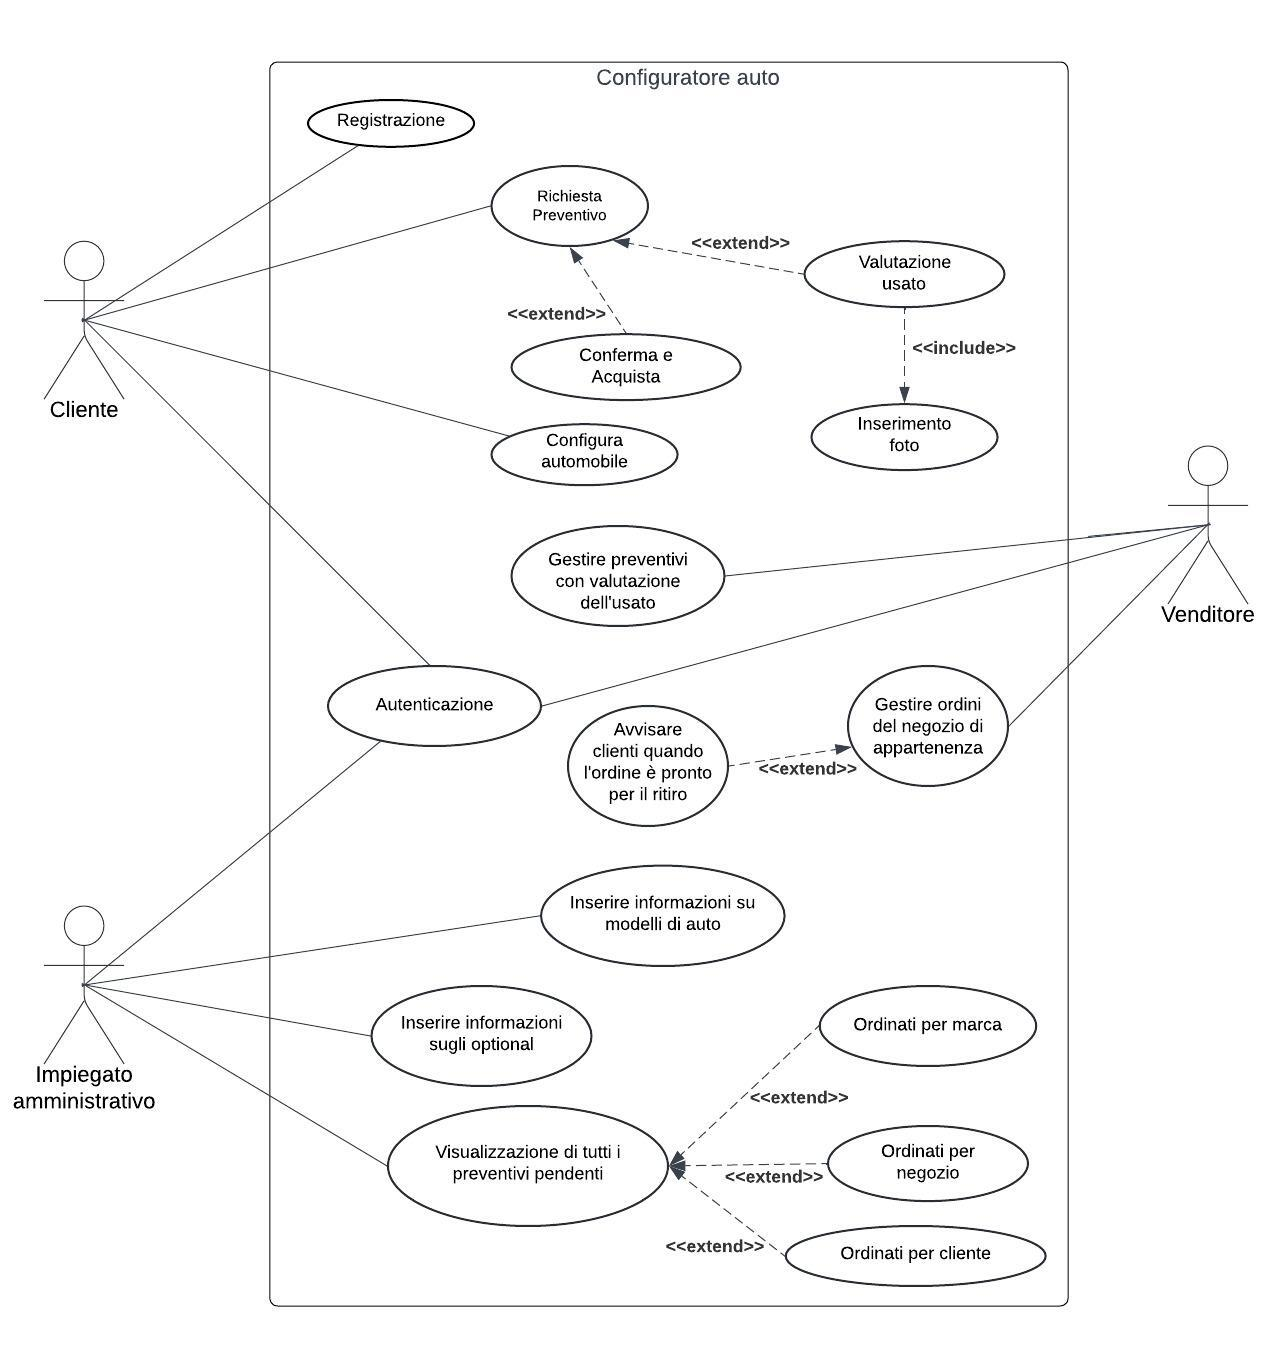
\includegraphics[scale=0.8]{UseCase}
\end{center}

\subsection{Casi d'uso relativi ai clienti}
\subsubsection{Configurare un'automobile}

Un cliente generico, anche non registrato, pu\`o utilizzare il sistema per configurare un'automobile.

\fbox{\defbox{
\itshape
\textbf{Precondizioni}: Nessuna. \\
\textbf{Attori}: Cliente. \\
\textbf{Passi}: 
\begin{enumerate}
\item \begin{enumerate}
		  \item Il cliente effettua la registrazione
		  \item Il cliente effettua l'accesso
		  \item Il cliente avvia la configurazione come ospite
	  \end{enumerate}
\item Il cliente seleziona dall'apposito menu la marca desiderata.
\item Il cliente seleziona dall'apposita tendina il modello desiderato.
\item Il cliente pu\`o scegliere una serie di optional aggiuntivi.
\begin{enumerate}
\item Se il cliente \`e nel sistema come ospite, viene portato alla scheramta di login / registrazione.
\begin{enumerate}
\item L'utente effettua il login.
\item L'utente effettua la registrazione.
\end{enumerate}
\item Se il cliente si \`e gi\`a autenticato, visualizza la schermata di riepilogo.
\end{enumerate}
\item Il cliente seleziona la sede di ritiro. 
\item Il cliente pu\`o proporre un usato da valutare per ottenere uno sconto.
\item Il cliente conferma la configurazione generata. 

\end{enumerate} 
\textbf{Postcondizioni}: L'automobile \`e configurata ed \`e possibile visualizzare il riepilogo nell'area utente.
\'E possibile confermare il preventivo.
}}
\mdseries

\subsection{Conferma dell'ordine}

Quando un'auto configurata viene confermata, l'utente pu\`o trovare il riepilogo nella sua area personale per 20 giorni.
In questo periodo \`e possibile confermare la configurazione, pagando l'acconto e generando l'ordine. Il caso particolare
di valutazione dell'usato prevede gli stessi passi, ma la visualizzazione nella lista dei preventivi \`e subordinata alla
conferma di un venditore della concessionaria di riferimento, che deve valutare l'usato e inserirne il valore, che verra'
automaticamente scontato dal prezzo finale dell'automobile configurata. Il preventivo legato alla valutazione verr\`a
visualizzato nella lista, con opportuna notifica, quando un venditore l'avr\`a preso in carico.

\fbox{\defbox{
\itshape
\textbf{Precondizioni}: Una configurazione provvisoria completata dal cliente. Cliente autenticato. \\
\textbf{Attori}: Cliente. \\
\textbf{Passi}: 
\begin{enumerate}
\item Il cliente, che si trova sulla home dell'area personale, seleziona dall'apposita tendina il preventivo dell'automobile
\item configurata e preme ``Apri''.
\item Il cliente viene portato sulla schermata di riepilogo dove pu\`o visualizzare la configurazione selezionata.
\item Il cliente conferma l'ordine cliccando sull'apposito pulsante ``Conferma e paga acconto''.
\item Il cliente visualizzer\`a la data prevista di consegna. 
\end{enumerate}
\textbf{Postcondizioni}: La configurazione viene spostata dai preventivi agli ordini.
}}
\mdseries

\subsection{Casi d'uso relativi ai Venditori}

\subsubsection{Valutazione dell'usato}
Un venditore di una concessionaria pu\`o accedere al sistema per valutare i preventivi con allegata richiesta di
valutazione dell'usato. Dopo opportuna autenticazione nel sistema, il venditore pu\`o richiamare la lista dei preventivi
pendenti inerenti al suo negozio di appartenenza. Il venditore a questo punto deve valutare l'usato, inserire nell'apposita interfaccia un importo, equivalente allo sconto che i cliente ricever\`a sull'automobile nuova che ha configurato.

\fbox{\defbox{
\itshape
\textbf{Precondizioni}: Autenticazione nel sistema da parte del venditore. Presenza di almeno un preventivo con richiesta
di valutazione dell'usato. \\
\textbf{Attori}: Venditore. \\
\textbf{Passi}: 
\begin{enumerate}
\item Il venditore visualizza le foto dell'auto nell'apposita interfaccia.
\item Il venditore inserisce un importo relativo al valore dell'automobile usata.
\item Il venditore conferma la valutazione.
\item Il venditore conferma il preventivo.
\end{enumerate}
\textbf{Postcondizioni}: Il preventivo \`e ora in attesa di conferma da parte del cliente.
}}

\mdseries

\subsubsection{Gestione degli ordini}

Il venditore gestisce gli ordini attivi per la sua concessionaria, occupandosi di avvisare i clienti quando le automobili
ordinate sono pronte per il ritiro.

\fbox{\defbox{
\itshape
\textbf{Precondizioni}: Accesso al sistema previa autenticazione. \\
\textbf{Attori}: Venditore. \\
\textbf{Passi}: 
\begin{enumerate}
\item Il venditore visualizza la lista degli ordini pronti per la consegna relativi alla sua sede.
\item Il venditore invia una notifica ai clienti con l'apposita funzione nell'area dedicata.
\end{enumerate}
\textbf{Postcondizioni}: Il cliente viene avvisato che l'ordine \`e pronto. L'ordine viene rimosso dal sistema e spostato
nella categoria ``ritiri''.
}}

\subsection{Casi d'uso relativi all'Amministrazione}

\subsubsection{Inserire un modello d'auto}

L'impiegato amministrativo \`e responsabile dell'aggiunta di nuovi modelli a catalogo. 

\fbox{\defbox{
\itshape
\textbf{Precondizioni}: Autenticazione. \\
\textbf{Attori}: Impiegato. \\
\textbf{Passi}: 
\begin{enumerate}
\item L'impiegato seleziona la funzione ``aggiungi auto''.
\item L'impiegato accede all'interfaccia di inserimento automobili.
\item L'impiegato seleziona la marca della nuova automobile.
\item L'impiegato compila i campi relativi alle informazioni di base del nuovo modello.
\item L'impiegato conferma l'inserimento.
\end{enumerate}
\textbf{Postcondizioni}: Il catalogo viene aggiornato con la nuova automobile.
}}

\subsubsection{Inserire nuovi optional}

L'inserimento di nuovi optional \`e analogo all'inserimento di una nuova automobile, con la differenza che l'impiegato deve accedere all'interfaccia ``Aggiungi optional''.

\subsubsection{Visualizzazione dei preventivi}

L'impiegato pu\`o accedere a tutti i preventivi pendenti presenti nel sistema. Ha la possibilit\`a di ordinarli per cliente, per marca o per negozio di consegna.

\fbox{\defbox{
\itshape
\textbf{Precondizioni}: Autenticazione. \\
\textbf{Attori}: Impiegato. \\
\textbf{Passi}: 
\begin{enumerate}
\item L'impiegato accede all'interfaccia di consultazione dei preventivi attraverso la funzione ``Visualizza preventivi''.
\item \begin{enumerate}
		\item L'impiegato ordina i preventivi per marca.
		\item L'impiegato ordina i preventivi per cliente.
		\item L'impiegato ordina i preventivi per negozio di ritiro.
		\end{enumerate}
\item L'impiegato visualizza il primo preventivo, secondo l'ordine selezionato.
\item L'impiegato, attraverso le apposite frecce, scorre i preventivi presenti nel sistema.
\end{enumerate}
\textbf{Postcondizioni}: Nessuna.
}}

\section{Diagrammi delle attivit\`a}


\chapter{Progettazione e implementazione}

\section{Note sul processo di sviluppo}

Il processo di sviluppo è stato di tipo agile incrementale ma suddiviso in tre sotto-processi distiniti. La prima parte ha permesso lo sviluppo del lato cliente nelle sue componenti principali, quali l'interfaccia di accesso e le procedure di registrazione di un nuovo utente; in contemporanea alla funzione principale del sistema, ovvero il configuratore auto vero e proprio. Dopo una fase di test l'attenzione si \`e spostata sulla proggettazione e lo sviluppo della parte dedicata al venditore, ad un sistema di preventivi e ordini.
La parte amministrativa \`e stata sviluppata per ultima perch\'e necessitava di un prototipo stabile alla base per poter essere implementata, inoltre le funzionalit\`a richiedevano i dati generati dalle categorie di utente generate in precedenza.
L'implementazione \`e ha seguito l'ordine di sviluppo necessario partendo dalle funzioni di base e aggiungendo mano a mano i layer successivi.

\section{Architettura del progetto}




\section{Desing Pattern}

\subsection{Note introduttive}

Il progetto nel suo insieme segue un desing pattern di tipo \textbf{Singleton}. Tuttavia, per la rappresentazione degli utenti nei tre sottotipi: cliente, venditore e impiegato, \`e stato usato un desing pattern di tipo \textbf{Decorator}; questo ha permesso di mantenere alcune funzionalit\`a generiche nella classetexttt{Utente}, estendendo e specializzando le tre sotto-classi \texttt{Cliente}, \texttt{Venditore} e \texttt{Impiegato}, relative agli acquirenti, ai venditori nelle sedi e algi impiegati amministrativi.

subsection{Singleton}

Il Singleton \`e usato per assicurare che una classe abbia una sola istanza per tutto il ciclo di vita del software e un unico punto di accesso globale. Le classi Singleton hanno costruttori privati per evitare la possibilit\`a di istanziare pi\`u oggetti della stessa classe. Esiste un metodo statico che fa in modo che nessuna istanza venga creata oltre alla prima, restituendo un riferimento a quella esistente.

Nella pratica, la classe Singleton del sistema software da noi prodotto \`e \texttt{SessionManager}, che riunisce una serie di metodi per gestire lo stato della sessione.  


\subsection{Decorator}

Il pattern Decorator permette di aggiungere funzionalit\`a ad un oggetto gi\`a esistente senza modificarne le propriet\`a o la struttura. Si crea una classe Decorator che fa da wrapper alla classe originale e aggiunge funzionalit\`a mantendo i metodi della classe intatti.

Nel sistema prodotto, la classe Decorator \`e \texttt{Utente}, che viene estesa da Cliente, Venditore e Impiegato. 










\end{document}